
\section{Niðurstöður}
\label{sec:nidurstodur}

Samkvæmt útreikningum okkar hefðu plöturnar gefið sig á undan boltunum eða við $4375 N$, sbr. kafla \ref{ch::reikningar}.
Boltarnir hefðu átt að þola allt að \fxnote{álag sem boltar þola} álag.


Við álagsprófið beygluðust stálplöturnar en boltarnir virðast ekki hafa orðið fyrir neinu hnjaski \fxnote{Skoða bolta!}.
Auk þess má sjá á stálplötunum að álagið var að mestu leyti á eina af ytri plötunum og því var átakið skakkt. Þetta olli því að meira af álaginu fór í stálplöturnar, en minna af álaginu í boltana. 
Það olli því að plöturnar beygluðust áður en nægt átak færi í boltana til að valda einhverju teljanlegu átaki á boltana.

Því má í rauninni segja að prófið hafi verið gallað þar sem tækin voru ekki nógu nákvæm til að setja álagið beint í boltana. Það olli því að plöturnar gáfu eftir mun fyrr en þær hefðu annars gert.

\begin{figure}[b]
  \centering
  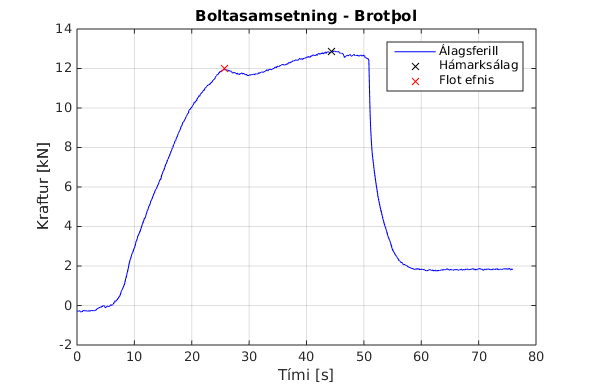
\includegraphics[width=\linewidth]{alag}
  \caption{Álagsferill í þolprófun}
  \label{fig:alag}
\end{figure}